\documentclass[a4paper]{article}

%% Language and font encodings
\usepackage[english]{babel}
\usepackage[utf8x]{inputenc}
\usepackage[T1]{fontenc}
\usepackage{caption}

%% Sets page size and margins
\usepackage[a4paper,top=3cm,bottom=2cm,left=3cm,right=3cm,marginparwidth=1.75cm]{geometry}
\usepackage[section]{placeins}
%% Useful packages
\usepackage{amsmath}
\usepackage{graphicx}
\usepackage[colorinlistoftodos]{todonotes}
\usepackage[colorlinks=true, allcolors=blue]{hyperref}

\title{Chapter 8 Autocorrelation Assignment}
\author{Petra Guy}

\begin{document}
\maketitle

\section{Introduction}
I have three scripts (so far!). Initially I wrote a python-ish functions script, 
but I wanted to make this run using Rscript, which I couldnt.
I therefore rewrote this as a long ugly code, thinking that if I ran that
from Rscript it would simple run through line by line. But the 
load command would not work. I also checked the results of my 
calculations against the R acf() function, and they were the same, 
so I wrote another script using that. 

\section{Graphs}


\begin{minipage}{\linewidth}
\begin{center}
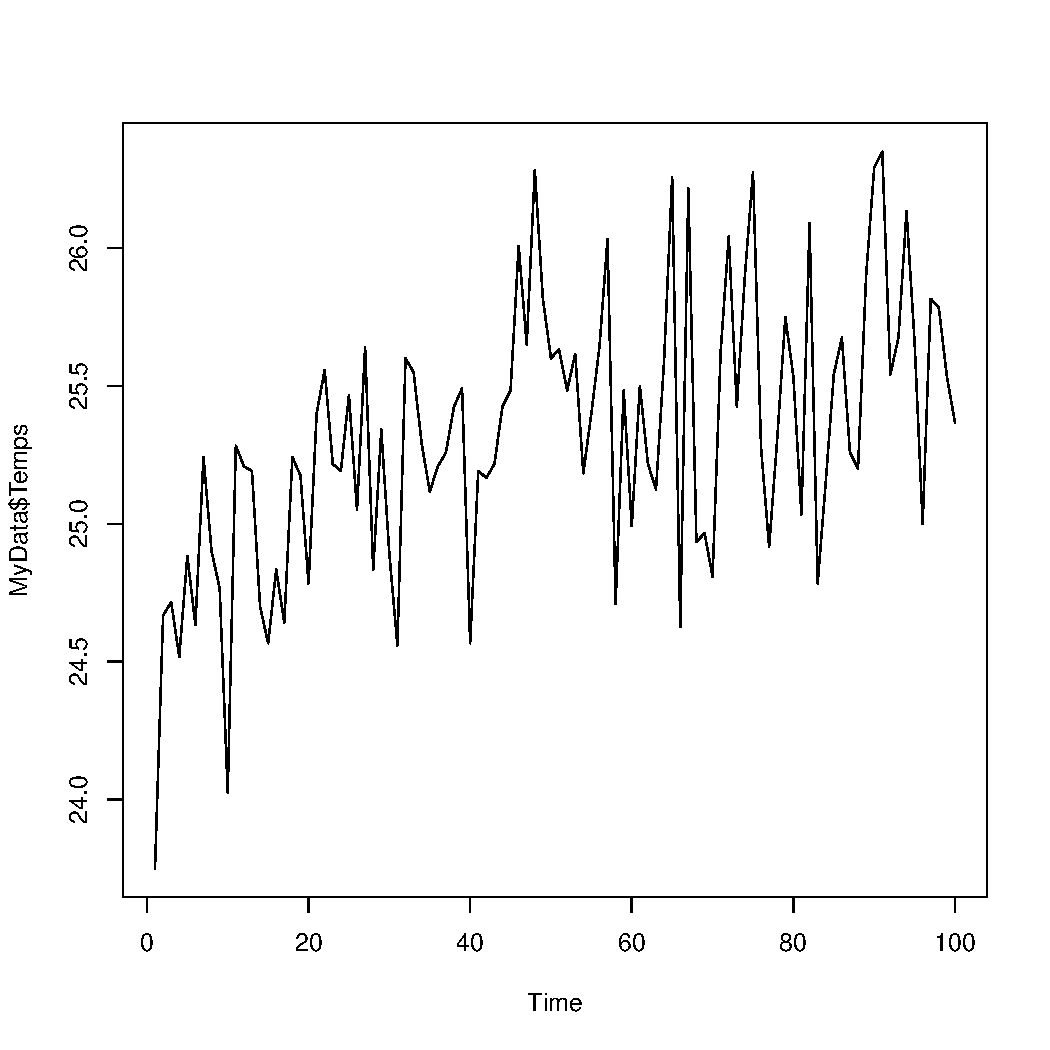
\includegraphics[width=.5\linewidth]{TAutocorrtimeseries1.pdf}
\captionof{figure}{Time series plot.}
\end{center}
\end{minipage}

\begin{minipage}{\linewidth}
\begin{center}
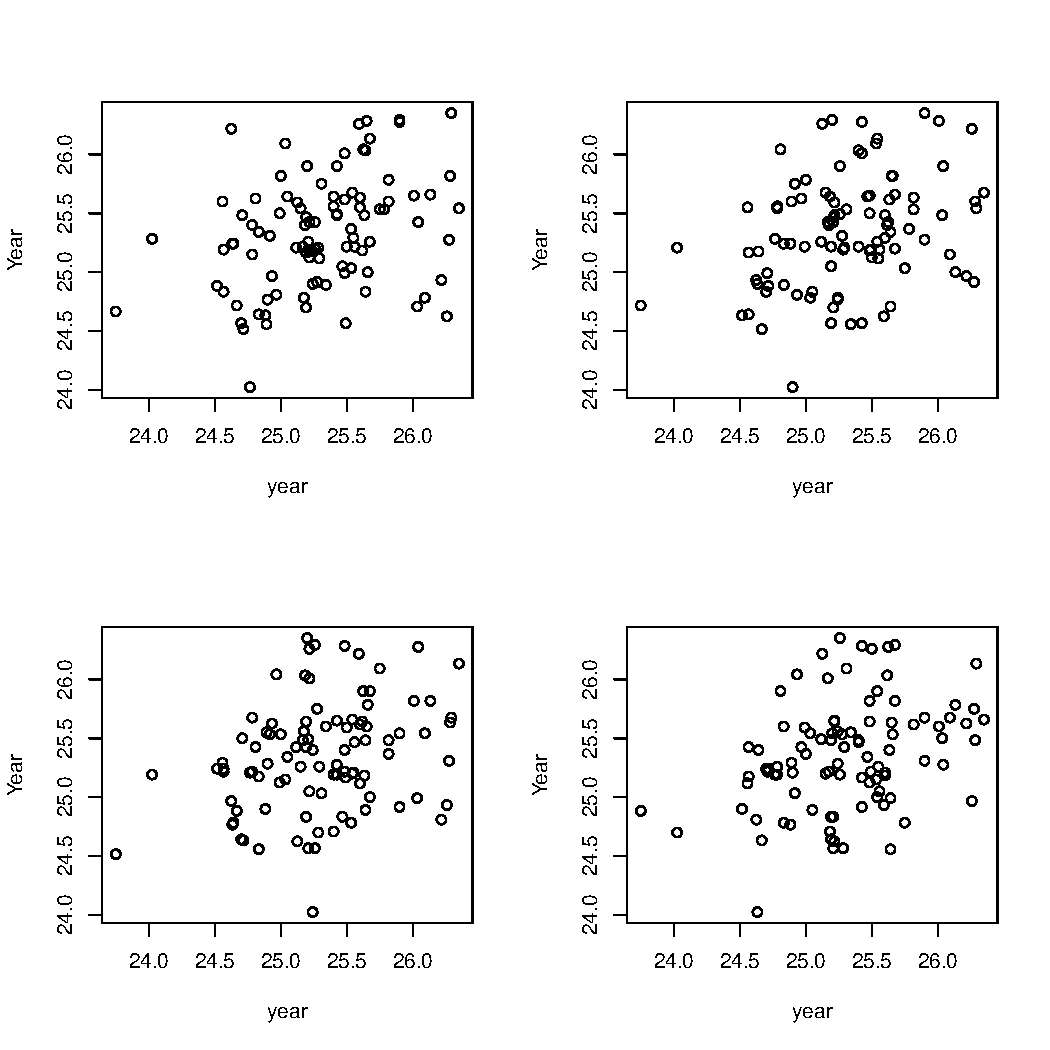
\includegraphics[width=.5\linewidth]{TAutocorrtimeseries2.pdf}
\captionof{figure}{Scatter plots of lag 1 to 4.}
\end{center}
\end{minipage}

\begin{minipage}{\linewidth}
\begin{center}
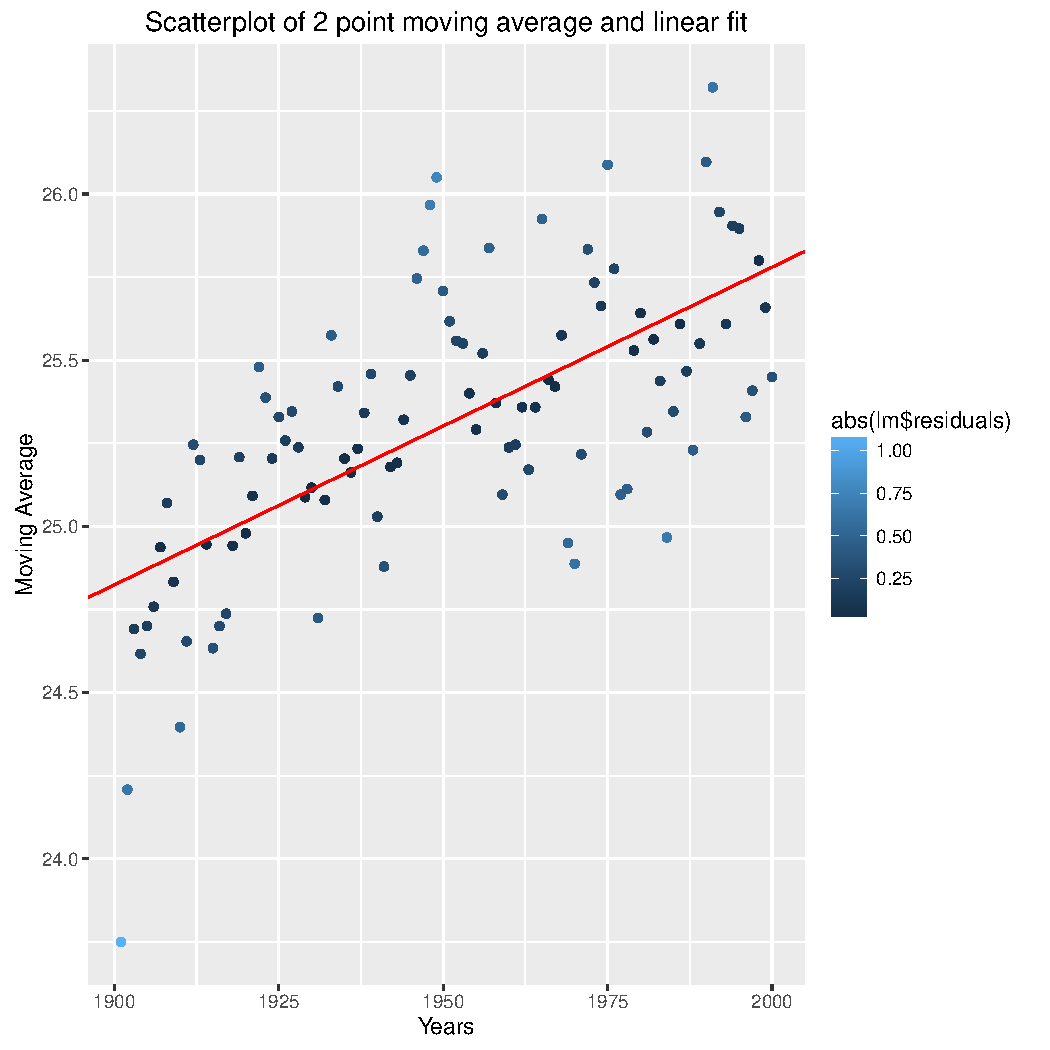
\includegraphics[width=.5\linewidth]{TAutocorrmovingavg.pdf}
\captionof{figure}{Moving Averages and straight line fit.}
\end{center}
\end{minipage}X

\end{document}
